%%%%%%%%%%%%%%%%%%%%%%%%%%%%%%%%%%%%%%%%%%%%%%%%%%%%%%%%%%%%%%%%%%%%%%%%
% Plantilla TFG/TFM
% Escuela Politécnica Superior de la Universidad de Alicante
% Realizado por: Jose Manuel Requena Plens
% Contacto: info@jmrplens.com / Telegram:@jmrplens
%%%%%%%%%%%%%%%%%%%%%%%%%%%%%%%%%%%%%%%%%%%%%%%%%%%%%%%%%%%%%%%%%%%%%%%%

\chapter{Marco Teórico}
\label{marcoteorico}
\par A continuación se expone la teoría necesaria para la comprensión de este \gls{tfg}, ampliando la información ya presentada en el capítulo \ref{introduccion}.
\section{Técnicas de regresión y Machine Learning}


\par Las técnicas de regresión proporcionan una estimación útil para realizar predicciones, por lo que están relacionados con el aprendizaje automático o \gls{ml}. El \gls{ml} es un tipo de inteligencia artificial, que se caracteriza por la generación de un modelo estimado de manera automática por un computador. Esta estimación se realiza con un entrenamiento previo aplicado a un algoritmo de aprendizaje específico a una serie de datos de entrenamiento. Con este aprendizaje se elabora un modelo que es capaz de devolver una salida o solución a partir de unos parámetros de entrada que deben ser del mismo tipo que los utilizados en la fase de aprendizaje. 
\\
\par * Introducir aquí esquema de ML *
\\
\par Finalmente, el objetivo de las técnicas de \gls{ml} puede ser clasificar una información o realizar una previsión acorde con un modelo estimado. Como se puede ver, el objetivo de este y las técnicas de regresión pueden coincidir y esto lleva a que tienen parte de su desarrollo en común. 

\subsection{Clasificación de técnicas de Machine Leaning}
\par Los modelos empleados en \gls{ml} son numerosos, y su clasificación se puede realizar dependiendo de su algoritmo de aprendizaje y del tipo de razonamiento en el que se basa. Comenzando por la clasificación según su algoritmo de aprendizaje, que principalmente se dividen según el feedback  del que aprenden, los modelos se pueden clasificar de la siguiente manera \cite{MLRussell}: 
\begin{itemize}
	\item Aprendizaje no supervisado: este aprendizaje se basa en la clasificación o agrupación de los objetos de entrada según patrones que cumplen las distintas entradas de estos. Estos métodos no devuelven un nombre específico para cada grupo o cluster ya que no se le han proporcionado referencias o etiquetas en la etapa de entrenamiento. Necesita numerosas entradas en el entrenamiento para detectar patrones suficientemente estables. 
	\item Aprendizaje por refuerzo: el aprendizaje se realiza por refuerzo positivo, que sería una recompensa, o negativo, penalización. Este algoritmo buscaría la estimación del modelo para obtener el máximo refuerzo positivo posible. Así, tras suficiente entrenamiento construye un modelo muy preciso para nuevas entradas. 
	\item Aprendizaje supervisado: tanto las entradas como las salidas están previamente definidas en la etapa de aprendizaje. Se realiza un entrenamiento en el que se utilizan las entradas con sus correspondientes salidas para elaborar el modelo. Una vez suficientemente entrenado, este puede obtener salidas previamente desconocidas a partir de entradas similares a las del entrenamiento. 
	\item Aprendizaje semi-supervisado: este aprendizaje recibe algunas de sus entradas correctamente etiquetadas y el resto de ellas, la mayoría, sin etiquetar, así tiene algunas referencias para la clasificación fiables pero no toma las etiquetas como una referencia totalmente cierta para toda la clasificación como ocurre en el aprendizaje supervisado. Así se evitan malos aprendizajes por ruido o etiquetas erróneas en los datos de entrada. Bastante común en grandes masas de datos para aprendizaje. 
\end{itemize}
\par Por otra parte, teniendo en cuenta la base de los razonamientos internos que los algoritmos realizan para obtener las salidas correspondientes, aunque no considerando esta división estricta, las técnicas se pueden clasificar de la siguiente manera \cite{MLFlach}:
\begin{itemize}
	\item Geométricos: los modelos geométricos son aquellos cuyos objetos pueden ser representados en un espacio de instancias (X) en el que cada instancia corresponde a un posible objeto, esto es, habrá tantas instancias como objetos con distintas combinaciones de entradas posibles. Por otra parte, las etiquetas también se representan como un espacio de etiquetas (Y) con un número finito de posibilidades \citep{MLPref}. Utilizando estos conceptos, el algoritmo se desarrolla con otros conceptos geométricos como son líneas, planos y distancias. Estos métodos suelen ser aplicados cuando X e Y están formados por valores numéricos, que son fácilmente representables en ejes de coordinadas.
	\item Probabilísticos: los modelos probabilísticos parten de la base de que las entradas de los objetos están basadas en un proceso aleatorio que hacen referencia a una distribución de probabilidad desconocida. Se busca definir esa distribución P(Y|X), siendo X el conjunto de objetos posibles e Y las etiquetas correspondientes. Aquí el modelo tendría como salidas probabilidades para cada una de las opciones posibles. 
	\item Lógicos: los modelos lógicos son los más cercanos al razonamiento humano y los más comprensibles también como algoritmos. Se basan en decisiones lógicas, estructuradas típicamente en forma de árbol, esto es llamado árbol de decisiones y según las características de los parámetros de entrada nos vamos desplazando hacia la base del árbol, obteniendo al final una única salida para cada objeto de entrada. *Introducir esquema*
	\item Agrupaciones y gradiente: estos modelos se incluyen en los anteriores, ya que es una clasificación paralela según el tratamiento del espacio de instancias (X): agrupaciones seccionando estos espacios en un número de segmentos definido, fácilmente representables y con una única solución, en cambio; en los gradientes, no existe una segmentación previamente definida, por lo que el modelo trata todo el espacio como uno solo. 
\end{itemize}

\subsection{Modelos de Machine Learning y aplicaciones}
\par Una vez presentadas todas las posibles clasificaciones de técnicas de \gls{ml}, podemos adentrarnos en los modelos más comunes, a qué tipo de los anteriores pertenecen y cuáles son sus aplicaciones más usuales y en las que son más efectivos. Algunos de los más conocidos son los siguientes:
\begin{itemize}
	\item Redes neuronales artificiales: este modelo es de tipo geométrico y de aprendizaje supervisado, ya que el entrenamiento consta de entradas etiquetadas con su correspondiente salida. Este modelo se caracteriza por estar inspirado por las redes neuronales naturales del cerebro animal, obteniendo resultados sin unas reglas preestablecidas de análisis. Estas redes están compuestas por capas de neuronas, las cuales representan un peso y una función de activación por la que una parte de la información de entrada se va a procesar. Estas funciones y pesos se van ajustando mediante el entrenamiento hasta tener una red óptima para su funcionamiento. En cuanto a aplicaciones, la más común de este modelo es el reconocimiento en imágenes de objetos o caracteres. Cuando analizamos imágenes cada unidad de información a la entrada para un objeto está formada por un pixel, y cada capa de neuronas irá reconociendo formas, colores, etc. hasta devolver la clasificación que corresponde a ese objeto de entrada. 
	\item Árboles de decisión: es un modelo lógico y de aprendizaje supervisado. Es lo de los modelos lógicos más ilustrativos porque se basa en árboles que siguen las reglas de decisión, yendo desde el primer nodo donde se sitúa la entrada resolviendo condiciones de estas hasta llegar a una única salida, alcanzable por un camino único, que es la salida del modelo. En el aprendizaje, este modelo va ajustando sus condiciones y elaborando el árbol más coherente para llegar a las soluciones necesarias. Este método es bastante sencillo de implementar y comprender, por lo que las aplicaciones son diversas. Relacionado con ese modelo también encontramos el conocido como \gls{rf}, anteriormente mencionado. Este modelo se caracteriza por generar numerosos árboles de decisión provenientes de un factor aleatorio con la misma distribución. Al obtener los resultados de cada uno de los árboles, se realiza un promediado, tomando la respuesta más repetida como la más probable y teniendo en cuenta el resto en su correspondiente porcentaje. De esta manera, un modelo que era limitado a una respuesta única, se abre devolviendo una respuesta probabilística. 
	\item Máquinas de vectores de soporte: es un modelo geométrico y supervisado. Este modelo geométrico utiliza el espacio de instancias para representar los objetos de entrenamiento como puntos y las clases o salidas como líneas o hyperplanos, dependiendo del número de dimensiones, lo más separados posibles unos de otros. Una vez ajustado este modelo, las nuevas entradas se clasificarán según al espacio al que pertenezcan. Este modelo está muy relacionado con la clasificación/agrupación y la regresión. Algunas de sus aplicaciones son el reconocimiento de caracteres escritos a mano \cite{MLhand} y clasificación de textos \citep{MLText}, la clasificación de imágenes por segmentación \citep{MLimg} o, el más interesante para este proyecto, la clasificación de información procedente de un \gls{sar} \citep{MLSAR}
	\item Redes bayesianas: es un modelo probabilístico y gráfico, a la vez que lógico, de aprendizaje supervisado. Se basa en un modelo gráfico de nodos que corresponden a variables conocidas o desconocidas y el tratamiento probabilístico simplificado con la regla de la cadena. Son muy utilizadas en aplicaciones relacionadas con las ciencias de la salud para modelar comportamientos biológicos. 
	\item Algoritmos genéticos: son algoritmos basados en la genética biológica. Estos comienzan con unas muestras aleatorias de posibles salidas, se evalúan y se realizan una serie de transformaciones que incluyen la selección de los mejores resultados, su recombinación y alteración de algunos para volver a empezar con la siguiente entrada, así hasta tener un modelo estable, fiable y calibrado. Este modelo se utiliza bastante para análisis y predicciones.
	\item También se consideran, entre otros métodos, los análisis de regresión. Técnicas que se pueden aplicar, como se puede ver en el siguiente apartado, al \gls{ml}, ya que comparten un mismo objetivo. 
\end{itemize}
\subsection{Análisis de regresión}
\par Las técnicas de regresión son todas aquellas técnicas que buscan la relación de una variable dependiente con una o más variables independientes mediante la estimación de su función de regresión. Para ello se consideran y ponderan todos los valores de la variable dependiente para unos valores fijos de las variables independientes. Además, en estos análisis, también se tiene en cuenta la varianza de la variable dependiente para estos mismos valores, pudiendo ser estudiada también mediante su distribución de probabilidad. Esta varianza indica la fiabilidad de nuestras estimaciones o el ``ruido'' en las medidas de la variable dependiente. 
\\
\par El caso más sencillo de regresión es en el que solo tenemos una variable dependiente y otra independiente, este caso se conoce como regresión lineal simple, ya que la función de regresión estimada se corresponde a una ecuación lineal de una recta. Los datos que obtenemos para la variable dependiente que vamos a relacionar tienen, aparte de las componentes lineales, una componente aleatoria de ruido que puede deberse a distintos fenómenos como la precisión mínima del instrumento de medida, el ruido que este mismo general en la medida o contribuciones de fuentes externas, consideradas como ruido también. Esta función de regresión es frecuentemente estimada mediante el \gls{mmc}. También existe la regresión lineal múltiple, que funciona de la misma manera pero con mayor número de variables independientes, por lo que en lugar de una recta, la función de regresión representa un plano en el que coinciden N dimensiones, siendo N el número de variables independientes total. Su expresión analítica se presenta en la ecuación \label{RL}, donde $Y$ corresponde a la variable dependiente, $X$ a las variables independientes, $\beta$ parámetro de influencia de cada variable independiente, y $\varepsilon$ el término aleatorio.
\\
\begin{equation} \label{RL}
Y_{t}=\beta _{0}+\beta _{1} X_{1}+\beta _{2} X_{2}+...+\beta _{N} X_{N}+\varepsilon 
\end{equation}
\par Cuando la función de regresión no es una función lineal, la regresión es no lineal, ya que la respuesta de la variable dependiente puede ser exponencial, logarítmica o polinomial, entre otras, por lo que la función de regresión presentará mayor complejidad. Aquí también es común utilizar el \gls{mmc} o la regresión segmentada, que ajusta como regresión lineal segmentos de la original no lineal.
\\
\par Cualquier variable independiente que tenga relación con la dependiente es útil en mayor o menor medida pero siempre proporciona información aunque su varianza sea muy grande o su contribución relativamente pequeña. Cualquier tipo de información extra proporciona un ajuste a la estimación final positivo si esta se ha modelado correctamente. 
\\
\par *Introducir aquí parte analítica regresión no lineal*
\\
\par A parte de las regresiones lineales y no lineales mencionados, también encontramos otros métodos de regresión como son los mínimos errores absoluto (bastante similar al \gls{mmc}), la regresión no paramétrica o la regresión lineal bayesiana.
\section{Teledetección}
\par Conociendo de qué trata este sector de las telecomunicaciones de una manera general, en este apartado se van a explicar conceptos más concretos de cómo funciona esta tecnología, qué tipos existen y qué técnicas se emplean en teledetección. 
\\
\par Como ya se menciona en el capítulo \ref{introduccion}, los instrumentos de teledetección se caracterizan por medir la radiación electromagnética emitida o reflejada por un objeto o superficie que se encuentra a distancia del mismo. Estos instrumentos se pueden clasificar en dos tipos: pasivos, miden la radiación natural emitida o reflejada por el objeto observado, o activos, emiten energía que posteriormente será reflejada y detectada.
\\
\par Algunos de estos instrumentos son cámaras fotográficas, láseres o radares. Todos ellos trabajan en un determinado rango en el espectro electromagnético, dependiendo de lo que quieran captar, por ejemplo los sensores ópticos necesitan trabajar en frecuencias del espectro visible, mientras que los radares pueden trabajar a frecuencias de microondas.
\subsection{Tecnología radar}
\par Para este proyecto nos vamos a centrar en el instrumento llamado radar. Se trata de un instrumento activo, que trabaja en el espectro de las microondas, concretamente entre 1-40 GHz. Por ello, son sensores sensibles a objetos del tamaño de sus longitudes de onda, es decir entre 30-0.75 cm, mucho mayores que los sensores ópticos. Además, otras ventajas frente a estos es su penetración en nubosidades e incluso parcialmente en la superficie terreste o la vegetación, por lo que, por ejemplo, el tiempo atmosférico, no supone un impedimento para la captación de información en la mayoría de los casos, como sucede en los sensores ópticos, y esto también se debe a la mayor longitud de onda.
\\
\par Al tratarse de un instrumento activo, este también ilumina con pulsos electromagnéticos el área a observar, emitidos por una antena propia, por lo que no depende de fuentes externas de radiación, esto es que, incluso objetos que no emitan radiación ni reflejen de otras fuentes, se podrán detectar gracias a la reflexión de esta incidencia. 
\\ 
\par La información que se obtiene en una antena receptora (o la misma emisora con doble función) de esta reflexión es otra onda electromagnética de la cual se puede medir su potencia, fase y polarización para obtener información útil del área observada. Para todas ellas deben tenerse en cuenta parámetros adicionales que influyen durante el trayecto del pulso, como es el retardo de fase o las pérdidas de potencia. El producto típico que esto genera se conoce como imagen \gls{sar}, es una representación gráfica cuyo eje horizontal corresponde al azimuth y el eje vertical al rango o distancia, y se presentan, normalmente en escala de grises, las contribuciones para cada ``pixel'', siendo el blanco la máxima y el negro la mínima. También se puede representar de igual manera la fase, en escala de grises o color, repartidos entre los 0-360º.
\\
\par La potencia recibida ($P_{R}$) se puede considerar como la contribución de los siguientes parámetros: potencia transmitida ($P_{T}$), longitud de onda ($\lambda$), ganancia de la antena ($G$), pérdidas en sistema ($L_{s}$) y en atmósfera ($L_{a}$), la longitud del trayecto ($R$), la superficie del área observada ($S$) y, por último, el coeficiente de backscattering ($\sigma_{0}$), teniendo en cuenta ambos trayectos de ida y vuelta y la propagación esférica de la onda, como se muestra en la fórmula \ref{Pr}. 
\\
\begin{equation} \label{Pr}
P_{R}=\frac{P_{T}\lambda ^{2}G^{2}\sigma_{0}S}{(4\pi ) ^{3}L_{s}L_{a}R^{4}}
\end{equation}
\\
\par Como podemos observar, el parámetro más interesante que nos va a dar información sobre el área observada es el coeficiente de backscattering. Este parámetro es un valor adimensional (dB) que representa la relación entre la proporción de área equivalente si el objeto observado fuera un blanco isótropo (reflexión total) ($m^{2}$) y su área o superficie observada real ($m^{2}$). Este parámetro va a depender de la frecuencia utilizada por el radar, la polarización de la onda, el ángulo de incidencia del pulso y del material y geometría de la superficie observada.
\\
\par Con el objetivo de maximizar la resolución espacial del área observada por el radar, esto es, la distancia mínima distinguible, se necesita mejorar la resolución en rango y en azimuth. La resolución en rango depende del tamaño del pulso, ya que los objetos podrán ser diferenciados si están a una distancia mayor que un pulso, por lo que cuánto más pequeño sea este, mayor resolución de rango se obtendrá, aunque se debe mantener la duración del pulso para el rango de frecuencias asignado. Por otra parte, para mejorar la resolución en azimuth, se debe incrementar la resolución angular. Esta resolución es inversamente proporcional al ángulo de observación, ya que cuanto mayor es este, más objetos o áreas considera a la misma distancia y no es posible diferenciarlos. Para obtener ángulos pequeños se necesita un swath, o haz de área iluminada, muy directivo, y ello se consigue con una apertura o longitud de radar grande. Es aquí donde entran los sistemas radar de los que se va a extraer la información para este proyecto, los \gls{sar}. Estos sistemas consiguen aumentar la resolución en azimuth, con una longitud no muy grande, realizando un barrido en azimuth y posterior procesamiento para ampliar el área observada sin compensar empeorando la resolución en azimuth. Un ejemplo de este barrido se puede ver en la figura \ref{fig:sarb}.
\\
\begin{figure}[h]
    \centering
    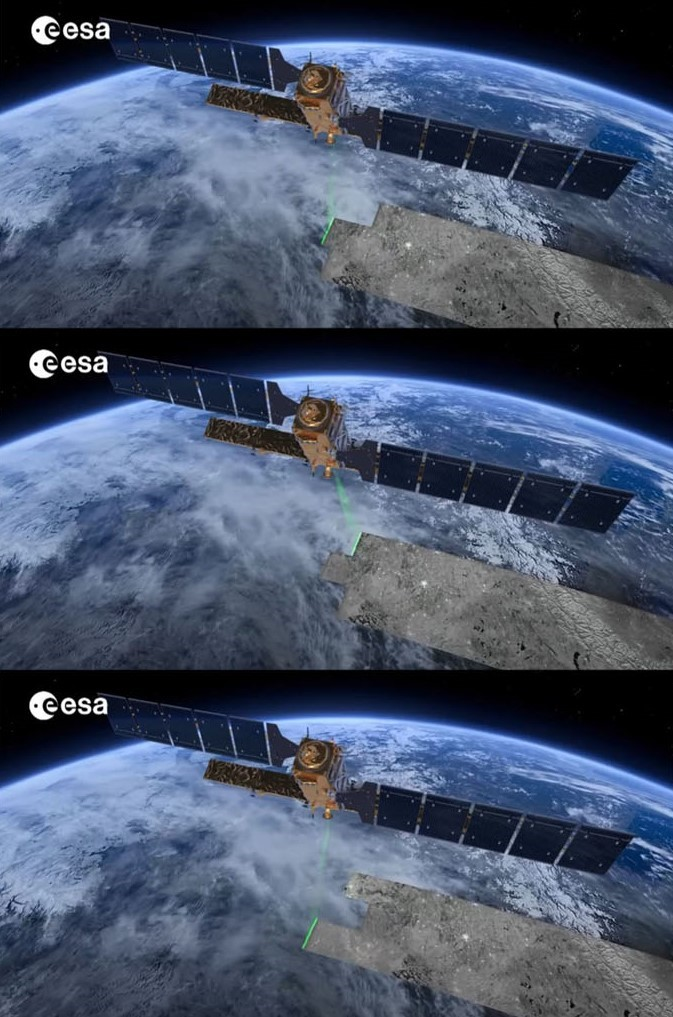
\includegraphics[height=12cm]{archivos/tfg/imgbarrido} % Tamaño de la imagen
    \caption{TOPS-SAR Sentinel-1 \cite{yts1}}
    \label{fig:sarb}
\end{figure}

\par Además de la resolución espacial, también existen otros parámetros que determinan la calidad de la información adquirida por los sistemas radar. Uno de ellos que aparece, similar al ruido blanco, como puntos de máximas y mínimas contribuciones debido a distintos fenómenos puede dificultar la interpretación de la información. Este ruido se denomina speckle, y la técnica utilizada para atenuar este efecto es la reducción por multi-look. Como su nombre indica, esta técnica se basa en la toma de varias imágenes de información de la misma área y el posterior promediado todas ellas, obteniendo una información más plana, viéndose reducidos los píxeles de información aleatorios máximos y mínimos. 

\subsection{Satélites en teledetección}
\par Los sistemas \gls{sar} van a ser utilizados en este proyecto para observar parcelas cultivadas de la Tierra, por lo que los sistemas en los que se van a emplazar estos son los satélites. Las misiones satelitales de las que se va a obtener información para este proyecto son Sentinel-1 y Sentinel-2, del Programa Copérnico de la \gls{esa}. Son dos misiones de órbita polar que engloban cada uno de ellos 2 satélites, A y B, cuyo objetivo es la observación de la superficie de la Tierra tanto terrestre como oceánica. Sentinel-1 concluyó sus lanzamientos de satélites en abril de 2016 y Sentinel-2 lo hizo en marzo de 2017. La principal diferencia entre estos dos es el rango de frecuencias de trabajo de cada uno, mientras que Sentinel-1  proporciona información de la banda C, esto es entre 4-8 GHz, Sentinel-2 utiliza tecnología multiespectral, por lo que trabaja en 13 bandas distintas, las cuales engloban la luz visible, el infrarrojo cercano y el infrarrojo de onda corta. Esto proporciona información más precisa y adecuada para cada fenómeno a observar \cite{copernicusOV}. 
\\
\par La órbita se traza en el eje polar de la Tierra con una pequeña inclinación y sincrónica al Sol, un periodo de revista global de 6 y 5 días y una altitud de 693 km y 786  km para Sentinel-1 y Sentinel-2, respectivamente y considerando ambos satélites, A y B, en ambos casos. En la figura \ref{fig:swath} se puede observar la órbita trazada por Sentinel-1 en un periodo de un día. Además, el sistema \gls{sar} no trabaja desde una posición perpendicular a la superficie terrestre a medir, ya que algunas superficies serían consideradas a la misma distancia por simetría en el swath, por lo que la visión del radar es lateral derecha. Esto deberá ser considerado para el procesamiento de extracción de información. 
\\
\begin{figure}[h]
    \centering
    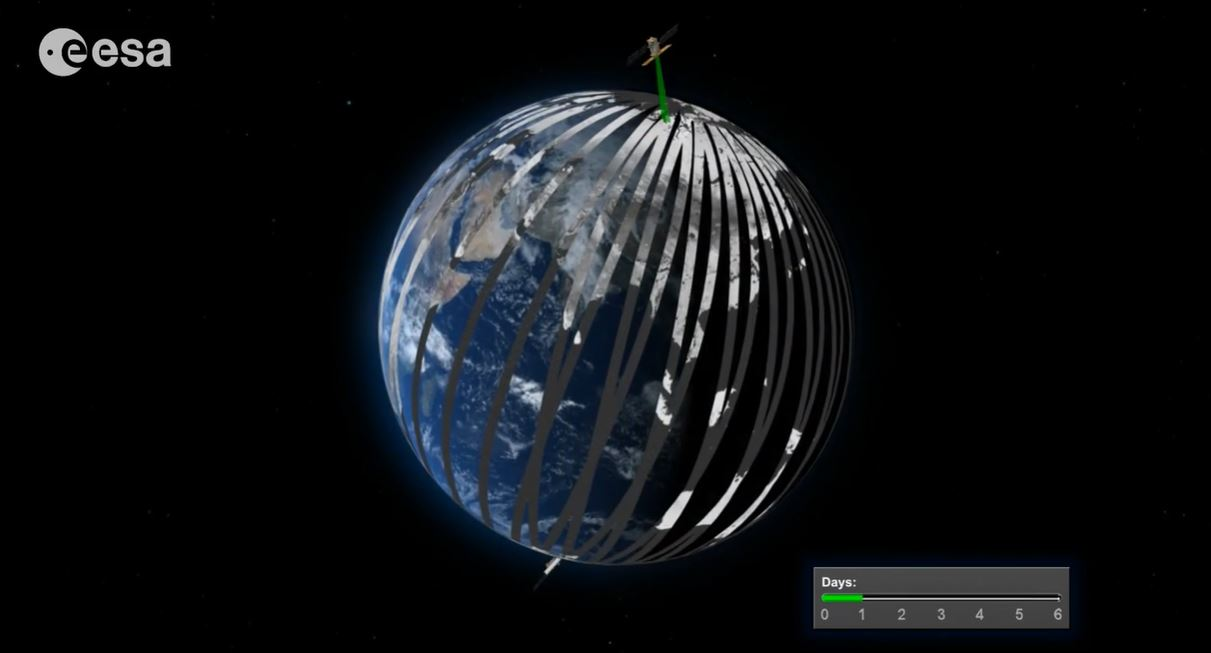
\includegraphics[height=7cm]{archivos/tfg/swathS1} % Tamaño de la imagen
    \caption{Swath a día 1 de 6 en Sentinel-1 \cite{ESAcons}}
    \label{fig:swath}
\end{figure}
\par Sentinel-1 tiene 4 modos de adquisición principales según el área que se pretende observar cuyos swath y resolución espacial varían. El primer modo, llamado Stripmap Mode, presenta un swath de 80 km y una resolución de 5x5 m. Este modo se utiliza para monitorización de islas pequeñas y emergencias puntuales. El segundo modo es Interferometric Wide Swath, de 250 km de swath y 5x20 m de resolución, es utilizado principalmente para todas las áreas de superficie terrestre, tanto áreas habitadas, como zonas montañosas o llanuras (donde se incluyen los cultivos). El tercer modo se conoce como Extra Wide Swath Mode, consta de un swath de 400 km y una resolución de 20x40 m, es utilizado para zonas marítimas, polares o cubiertas de hielo, donde se buscan grandes coberturas y un tiempo de revista corto, ya que, por el eje elegido para su órbita, las zonas polares se cubren en menor tiempo. Por último, cabe destacar el Wave Mode, cuyo swath se caracteriza por considerarse de superficie cuadrada de 20x20 km, y con una resolución de 20x5 m. Este es utilizado para la observación de los océanos \cite{EOSs1}. 
\\
\par Para que la utilización de estos modos sea posible, se necesita una tecnología \gls{sar} acorde con estas necesidades. El radar tiene unas dimensiones en Sentinel-1 de antena de 12.3 m x 0.821 m una vez desplegado. El rango del ángulo de incidencia con respecto a la Tierra es de 20”-46”. Los modos de adquisición también pueden trabajar con distintas polarizaciones. Las ofrecidas por los satélites de Sentinel-1 para la emisión son Horizontal (H) y Vertical (V). Para la recepción se pueden elegir la misma polarización utilizada en emisión, lo que sería HH o VV, o recibir ambas polarizaciones independientemente de cuál haya sido enviada, HH+HV o VV+VH \cite{EOSs1}. Una emisión con polarización doble entorpecería el procesamiento ya que no se podría reconocer en la recepción qué parte de la señal correspondía a cada una. 


\subsection{Técnicas de detección}
\par Con el objetivo de que la información captada por el radar sea comprensible y refleje una información coherente, existen distintos tipos de técnicas de detección según el tipo de información que se quiera extraer. Teniendo en cuenta solamente el coeficiente de backscattering en los sistemas \gls{sar} y la longitud de onda empleada ($\lambda$), ya existen ciertos rangos que suelen representar distintos tipos de superficies observadas:
\begin{itemize}
	\item $\sigma_{0}$ > 0 dB: típicamente objeto artificial liso que está encarado al ángulo de incidencia del radar y actúa como un espejo.
	\item -10 dB < $\sigma_{0}$ < 0 dB: superficies muy rugosas como pueden ser vegetaciones densas donde hay mucha probabilidad de reflexión.
	\item -20 dB < $\sigma_{0}$ < -10 dB: superficies rugosas como vegetaciones menos densas entre las que se incluirían los cultivos. 
	\item $\sigma_{0}$ < -20 dB: superficies lisas que no encaran el haz de incidencia del radar por lo que reflejan casi todo a otra dirección, esto se da en masas de agua en calma, carreteras o suelos muy secos. 
\end{itemize}
\par Por otra parte, existen técnicas de detección más complejas que consideran también la información proveniente de la fase y la polarización para el desarrollo de modelos. Los principales son:
\begin{itemize}
	\item Interferometría: técnica que toma en consideración la fase obtenida en cada medición como la contribución del trayecto de la señal, el desfase introducido en el procesado y el cambio de fase debido a la reflectividad de la superficie observada. Crea modelos topográficos a partir de las diferencias de fase para una misma área con posiciones distintas de radar (pequeños desplazamientos o variaciones de posición en cada ciclo). Las fases podrán ser útiles si existe una correlación entre ellas, es decir, si son coherentes.
	\item Interferometría diferencial: tiene como objetivo recrear un modelo topográfico temporal que represente las deformaciones del terreno con el paso del tiempo. Se basa en el mismo principio que la técnica anterior, ya que utiliza la diferencia de fase, primero entre dos imágenes para crear el modelo topográfico, y, a continuación, con una tercera para detectar las zonas de la superficie en las que ha habido un desplazamiento. También se puede realizar utilizando un modelo digital del terreno que aporta la topografía, y la diferencia de fase de dos imágenes para los desplazamientos. 
	\item Polarimetría: se basa en la polarización de la onda recibida como fuente de información. Analiza su polarización estudiando su orientación y elipticidad media, con ellas se obtienen las matrices o vectores de scattering que definen una superficie por el cambio que esta realiza a la polarización de una onda incidente polarizada conocida. Esto da información sobre el tipo de superficie que se está observando. 
\end{itemize}
\section{Estimación de parámetros físicos de cultivos mediante regresión}
\par A continuación, se van a presentar los conceptos físicos que definen el estado de desarrollo de los cultivos, para comprender cuáles son los parámetros clave y objetivos de este proyecto. Posteriormete, se expone la información útil extraíble de las imágenes \gls{sar}, a partir de la cuál se va a trabajar para el objetivo anterior. Por último, se verá la aplicación de las técnicas de regresión a los datos obtenidos para elaborar un modelo representativo del estado fenológico de un cultivo.

\subsection{Parámetros físicos de la fenología}
\par La fenología es la ciencia que estudia la relación entre los factores climáticos y los ciclos de los seres vivos \citep{feno}. Esto es, el estudio del desarrollo de plantas y animales en relación con parámetros ambientales. Este proyecto se centrará en el estudio fenológico de plantas, en concreto de cultivos de arroz, por lo que se va a profundizar en las características fenológicas que los describen. Algunos de los parámetros clave son los siguientes: 
\begin{itemize}
	\item Escala \gls{bbch}, que recibe su nombre por los participantes en su estudio y desarrollo, es una escala numérica de intervalo 0-9 que representa el estado de desarrollo fenológico de las plantas \cite{bbch}. Cada valor numérico corresponde a un estado de desarrollo, desde la germinación o primeros brotes, correspondientes al estado 0, hasta la senectud, estado 9. Cada estado puede estar dividido hasta en 10 sub-etapas. El rango de que cada etapa abarca, concretamente para los cultivos de arroz, se puede observar en la tabla *insertar tabla* \cite{bbcht}. Para que uno de estos estados sea considerado el nivel general de una parcela, no solo tiene que ser este estado el mayoritario, sino que debe abarcar más del 50\% del cultivo. 
	\item \gls{ndvi}, enunciado anteriormente, es el índice de vegetación de diferencia normalizada, es un índice usado para estimar la cantidad, calidad y desarrollo de la vegetación con base a la medición de la intensidad de la radiación de ciertas bandas del espectro electromagnético en ella. Estas bandas son concretamente las bandas del rojo y del infrarrojo cercano, con rangos de  reflexión entre 0 y 1 cada una de ellas. El coeficiente gls{ndvi} se obtiene según la fórmula \ref{eq:ndvi}, conformando un rango entre -1 y 1, y representa el desarrollo de la vegetación, ya que la contribución de la banda infrarroja cercana está ligada a la reflexión de la celulosa, por tanto a las áreas verdes y frondosas, mientras que la banda roja es mucho menos sensible a estas contribuciones y más a la absorción de clorofila. En resumen, un buen desarrollo vegetal tiene valores de \gls{ndvi} más cercanos a la unidad positiva \citep{ndvi}. 
	\begin{equation} \label{eq:ndvi}
		NDVI = \frac{IRCercano-ROJO}{IRCercano+ROJO}
	\end{equation}
	\item La altura del cultivo, aunque depende del tipo que sea, también es un indicador fiable del desarrollo de las plantaciones, sobre todo en cereales como, en este caso, es el arroz. El arroz, desde que germina hasta el momento de su cosecha, puede crecer entre 30-40 cm de alto según la variedad que este sea, por lo tanto, el seguimiento de la altura es un proceso sencillo y eficaz para monitorizar el estado de estos cultivos. 
	\item Temperatura del aire, o el calor acumulado durante todo el proceso de desarrollo de un cultivo, tiene influencia de manera directa en la duración de los distintos estados fenológicos del mismo. Concretamente en los cultivos de arroz tiene un impacto notable, por lo que se considera otro de los parámetros a tener en cuenta para su monitorización y en la elaboración de modelos de predicción \cite{Juanma2016}.
\end{itemize} 
\subsection{Extracción de información de imágenes \gls{sar}}
\par Las imágenes \gls{sar} dan una información de el coeficiente de reflexión de la superficie observada, según una polarización de onda emitida y recibida, siendo este representado en ejes de azimuth y rango, como se ha explicado anteriormente. Para este proyecto se van a tener en cuenta estas imágenes, de libre acceso por la \gls{esa}, con los canales de polarización VV y VH, esto es, emisión vertical y recepción tanto vertical como horizontal. Se ha elegido la polarización vertical ya que es la que el programa de los satélites de Sentinel-1 ofrece sobre Europa, y, además, es más sensible al crecimiento de los cultivos de arroz por la verticalidad de sus tallos. Por otra parte, las imágenes de polarización horizontal recibida proporciona información extra que puede ser útil y que es bastante semejante a la obtenida en HV, es decir, emisión horizontal y recepción vertical, por lo que se abarca la mayor parte de información útil posible. 
\\
\par Las imágenes \gls{sar} pueden ser adquiridas con distintos formatos. El que se va a utilizar aquí es el formato \gls{grd} *¿Resolución?* por conveniencia para este estudio. Este formato consiste en imágenes \gls{sar} multi-look (reducción de speckle) y proyectadas al rango de la tierra utilizando un modelo de elipsoide de la Tierra. La información de la fase es suprimida, lo cual no es un problema para este estudio, ya que no era uno de los parámetros clave, y los píxeles que presenta la imagen son aproximadamente cuadrados \cite{copData}. 
\\
\par El primer problema reconocible en la obtención de estas imágenes es su falta de correspondencia con las coordenadas geográficas comúnmente utilizadas, además de las dimensiones y orientación de estas, ya que las imágenes abarcan áreas de mucho mayor tamaño a las áreas de cultivos aquí estudiados, y la orientación no es totalmente paralela al eje polar de la Tierra, sino que presenta cierta inclinación. Para solucionar todo ello, se realiza un pre-procesado desarrollado por el Departamento de Física, Ingeniería de Sistemas y Teoría de la Señal de la Escuela Politécnica Superior, utilizando el software libre SNAP cedido por la \gls{esa}, que se divide en los siguientes pasos:
\begin{enumerate}
	\item Lectura de las imágenes.
	\item Actualización de la información orbital en las imágenes cargadas.
	\item Cancelación de ruido térmico.
	\item Recorte del área de interés.
	\item Calibración radiométrica para obtener de salida de ambos canales (VH y VV) el formato $\sigma_{0}$.
	\item Filtrado de speckle.
	\item Conversión de escala lineal a dB.
	\item Geo-referenciación: genera un mapa en una rejilla uniforme de
coordenadas cartográficas con tamaño de píxel elegido de aproximadamente 10 m para cada coordenada (latitud y longitud).
	\item Escritura del producto en formato propio de SNAP: DEAM-DIMAP 
\end{enumerate}
\par Esto se realiza tantas veces como número de imágenes de distintas fechas se hayan obtenido. Para finalizar el procesamiento, se ajustan unas imágenes con otras para que todas estén referenciadas a las mismas coordenadas cartográficas en los mismos píxeles. 

\subsection{Regresión aplicada a la estimación}